\section{Backgrounds}
\label{sec:od_analysis_backgrounds}
\par
Using the aforementioned energy scale, noise cut, and scaling factor, in this section, the background rate in the OD is measured, and attempts are made to understand the features observed in the data.
\par
In \autoref{fig:od_random_trigger}, a comparison between the observed events in the OD during the entirety of the first science run (SR1) from the Random Trigger (described in \autoref{sec:lz_detector}) and those expected are shown.
The expected rates are those described in \autoref{sec:simulated_od_requirements} and were simulated using the optical photon full-chain framework (described in \autoref{sec:lz_detector}) with the resultant pulse areas scaled by a factor of 4.54.
Both data and simulations were handled by the same analysis tools, with the noise cut applied.
Included as well in \autoref{fig:od_random_trigger} is the expected rate in the OD if the GdLS had not undergone an improved purification.
All three distributions are normalised to exposure.
Neither the improved purification nor the original purification fits what is observed particularly well.
More worryingly, there is a peak in the data at 100 phd, which is not present in either of the expected distributions.
The peak in the green data is from the $^{238}$U decay chain, which is the background most greatly reduced by the GdLS improved purification (see \autoref{tab:gdls_assay_rates}).
\par
In the remainder of this section, an effort is made to understand what is observed and why it differs from what was expected from radioassays and simulations.

\begin{figure}[]
    \centering
    \begin{tikzpicture}
    
    \begin{axis}[
        xlabel=Pulse Area,
        ylabel=Rate (Hz/5phe),
        width=15cm, height=10cm,
        xmin=0, xmax=1000,
        %ymax=1e-7, 
        ymode=log,
        legend pos=north east,
        grid=major]
            
        \addplot[only marks, mark size=0.5pt,
                 error bar legend,] 
            plot[error bars/.cd, x dir=both, x explicit]
            table[x=pulsearea,y=weight,x error=xerror, y error=yerror]
            {Data/OD_Backgrounds/background_constraints/od_data.dat};
        
        \addplot[red, const plot]
            table [x=pulsearea,y=weight]
            {Data/OD_Backgrounds/background_fit/starting_point/backgrounds_improved_purification.dat};
            
        \addplot[green, const plot]
            table [x=pulsearea,y=weight]
            {Data/OD_Backgrounds/background_fit/starting_point/backgrounds_original_purification.dat};
        
        \legend{Data, Original purification, Improved purification};
        \end{axis}
    \end{tikzpicture}
    \caption{OD pulse area spectrum from using the Random Trigger in the region. 
    Only the noise cut has been applied to the data.
    Overlaid are the expected rates from all backgrounds with the improved and original GdLS internal rates.}
    \label{fig:od_random_trigger}
\end{figure}


\subsection{Rate Stability}
\par
To begin the journey of understanding what is in the data, the first check performed was to observe if the rate and distribution of backgrounds were stable over time.
The OD was filled in June 2021, but between then and around the start of SR1 in December 2021, the electronic parameters of the detector were continuously altered during the commissioning phase.
As such, an OD background rate measurement only became stable around and during SR1.
Weekly monitoring of the OD was performed, starting from a month before the beginning of SR1 and running until the end of SR1, using the Random Trigger.
The rate of events above the noise cut, 100~keV, and 200~keV was measured and is shown in \autoref{fig:OD_SR1_Rate}.
The noise cut was applied as a base cut, so the 100~keV is made up of the noise cut plus a pulse area cut, and similarly for 200~keV.
The three gaps in the data are when calibrations were being performed.
This occurred three times in the region shown: just before SR1, four weeks into SR1, and straight after SR1.
\par
There are minor fluctuations in the noise cut rate, but these are linked to a xenon chiller and consistent with a grounding failure.
Importantly, over this period, the OD rate remains stable, with no features in the observed pulse area distribution changing during the monitored time.
Therefore what was shown in \autoref{fig:od_random_trigger} is considered representative of the backgrounds in the OD.
\par
Viewing the rate in a slightly different way, the rate-per-phd for the SR1 period is shown in \autoref{fig:od_sr1_rate_vs_threshold}.
Overlaid is the expected backgrounds rate from \autoref{tab:od_expected_rates} for 100 and 200~keV.
Interestingly the rate above 100~keV is in fairly good agreement with what was predicted in \autoref{sec:simulated_od_backgrounds}.
This is consistent with setting the veto energy threshold to 100~keV, assuming that achieves an appropriate veto efficiency.
However, differences arise at the 200~keV level, where the expected rate is 62.7$\pm$5.3~Hz whilst the observed rate is 42.5$\pm$2.1~Hz, a fairly significant difference.
This indicates that there are fewer backgrounds in the OD than expected, and therefore a veto energy threshold of 200~keV would have a lower false veto rate than expected by simulations for any veto time window.
%This is consistent with the result from full chain simulations, but the background components which make up the distribution are clearly different.

\begin{figure}[!htbp]
    \centering
   \begin{tikzpicture}
        \begin{axis}[
        date coordinates in=x,
        %xtick=data,
        xticklabel style=
        {rotate=90,anchor=near xticklabel},
        xticklabel=\day.\month.\year,
        xlabel={Date},
        %ymin=247, ymax=250,
        y tick label style={/pgf/number format/1000 sep=},
        extra y tick style={grid=major, tick label style={xshift=-1cm}},
        ylabel={Rate (Hz)},
        date ZERO=2009-08-18,% <- improves precision!
        width=15cm,
        height=6cm,
        ]
        \addplot[smooth, error bar legend,
                 error bars/.cd,
                 y dir=both, y explicit, error bar style={color=orange}] table[x=date,y=noise, y error=noise_error] {Data/OD_Backgrounds/background_rates/random_trig_rates.txt};
                 
        \addplot[smooth, error bar legend,
                 error bars/.cd,
                 y dir=both, y explicit, error bar style={color=orange}] table[x=date,y=100kev, y error=200kev_error] {Data/OD_Backgrounds/background_rates/random_trig_rates.txt};
        
        \addplot[smooth, error bar legend,
                 error bars/.cd,
                 y dir=both, y explicit, error bar style={color=orange}] table[x=date,y=200kev, y error=200kev_error] {Data/OD_Backgrounds/background_rates/random_trig_rates.txt};
                 
        \end{axis}
    \end{tikzpicture}
    \caption{Rate in OD during and before SR1 data taking on a week-by-week basis using the Random Trigger.
    Week -1 corresponds to the month prior to SR1 when the OD PMT gains were higher.}
    \label{fig:OD_SR1_Rate_spare}
\end{figure}
%\par


\begin{figure}[!htbp]
    \centering
    \begin{tikzpicture}
        \begin{axis}[
            title=TODO: Replace with dates and errors,
            xlabel=Data taking week,
            ylabel=Rate (Hz),
            width=15cm,
            height=6cm,
            xmin=-2,
            xmax=14,
            legend style = {column sep = 10pt, legend columns = -1,}]
            \addplot[red, only marks]
                    table [x=Week,y=Rate]
                    {Data/OD_Backgrounds/background_rates/od_sr1_rate_noise.dat};
            \addlegendentry{Noise Cut};
            \addplot[blue, only marks]
                    table [x=Week,y=Rate]
                    {Data/OD_Backgrounds/background_rates/od_sr1_rate_100.dat};
            \addlegendentry{100keV};
            \addplot[green, only marks]
                    table [x=Week,y=Rate]
                    {Data/OD_Backgrounds/background_rates/od_sr1_rate_200.dat};
            \addlegendentry{200keV};
        \end{axis}
    \end{tikzpicture}
    \caption{Rate in OD during and before SR1 data taking on a week-by-week basis using the Random Trigger.
    Week -1 corresponds to the month prior to SR1 when the OD PMT gains were higher.}
    \label{fig:OD_SR1_Rate}
\end{figure}

\begin{figure}[]
    \centering
    \begin{tikzpicture}
        \begin{axis}[
            xlabel=OD Threshold (phd),
            ylabel=Rate (Hz),
            width=15cm, height=8cm,
            xmin=-1, xmax=55,
            ymin=0, ymax=350,
            legend pos=north east,
            grid=major]
             \addplot+[black, smooth, mark=none]
                    table [x=Threshold,y=Rate]
                    {Data/OD_Backgrounds/background_rates/od_sr1_rate_vs_threshold_smooth_line.dat};
            \addplot[black, only marks, 
                     error bar legend,
                     error bars/.cd,
                     x dir=both, x explicit, error bar style={color=black}]
                    table [x=Threshold,y=Rate, x error=XError]
                    {Data/OD_Backgrounds/background_rates/od_sr1_rate_vs_threshold_error_bars.dat};
             \addplot[dashed, mark=none, red] coordinates {(0,100) (60,100)};
             \addplot[dashed, mark=none, blue] coordinates {(17.6,0) (17.6,350)};
             \addplot[dashed, mark=none, green] coordinates {(37.5,0) (37.5,350)};
             
             \addplot[orange, only marks, 
                      error bar legend,
                      error bars/.cd,
                      y dir=both, y explicit, error bar style={color=orange}]
                      table [x=Threshold,y=Rate, y error=YError]
                      {Data/OD_Backgrounds/background_rates/od_sr1_rate_expected.dat};
             
             \legend{,SR1 Data,$<$100Hz Requirement,100 keV (17.6 phd),200 keV (37.5 phd),Expected}                
        \end{axis}
    \end{tikzpicture}
    \caption{Rate of OD backgrounds during SR1 using the Random Trigger. The noise cut has been applied. 100Hz Requirement is for a 500$\mu$s veto window as proposed in \cite{LZ_TechnicalDesignReview_ref}. Expected values are from \autoref{tab:od_expected_rates}}
    \label{fig:od_sr1_rate_vs_threshold}
\end{figure}

%%%%%%%%%%%%
\subsection{Position Reconstruction}
\par
Next, we can look at the spatial distribution of events.
For any pulse, it is possible to estimate the location of the interaction that caused the pulse by a weighted average such as:
\begin{equation}
    x = \frac{\sum{\text{C}_{\text{phd}} \cdot \text{C}_\text{x}}}{\sum{\text{C}_\text{phd}}} 
\label{eq:OD_xy_position}
\end{equation}
where C$_{phd}$ is the phd of a PMT channel and C$_{x}$ is the physical position of the PMT.
In spherical coordinates, $\phi$ can be calculated in a similar fashion using the $\phi$ position of each PMT, Ch$_\phi$:
\begin{equation}
    \phi = \text{arctan}\bigg( \frac{\sum{\text{C}_\text{phd} \cdot \text{cos}(\text{C}_{\phi})}}{\sum{\text{C}_\text{phd} \cdot \text{sin}(\text{C}_{\phi})}} \bigg)
\label{eq:OD_phi_position}
\end{equation}
\par
Due to scheduling constraints associated with SR1, there was an insufficient variety of calibration sources used at varying \{$x,y,z$\} positions in order to adequately determine the resolution of this approach, but it is something a future calibration campaign may be able to tackle. 
Additionally, this approach does not consider the OCV in the centre of the detector, so reconstructed pulses will have an incorrect position, but the correct shape\footnote{Pulses can be reconstructed to \{0,0\} which is not physical as that is where the OCV is.}.
The OCV can be taken into account by including an offset in \{$x,y$\}, but this has explicitly not been done here due to the lack of knowledge in the resolution of this approach.
Regardless, this approach provides an insight in a way not thought possible based upon optical photon simulations\footnote{Due to the low light collection efficiency in the simulations.}.

\par
Spatial reconstruction was performed on slices in phd-space, the result of which can be seen in \autoref{fig:od_backgrounds_position_reconstruction}.
The first region focuses on the unexplained peak at 100~phd ($\backsim$~0.5~MeV).
The second region focuses on the area above 500~phd ($\backsim$~2~MeV), where cavern-$\gamma$s should dominate.

\begin{figure}[!htbp]%
\centering
\begin{tikzpicture}
\centering
  \begin{groupplot}[%view={0}{90},
    group style = {group size = 2 by 3,vertical sep=3cm,
                   horizontal sep=1.5cm},
                   height=6cm, width=0.5\textwidth]
    \nextgroupplot[
            ylabel=Rate (Hz),
            xlabel=Pulse Area (phd),
            width=0.95\textwidth,
            height=6cm,
            %xshift=0.5\textwidth,
            xmin=0, xmax=800,
            ymin=1e-4, ymax=1e3,
            ymode=log,
            ]
            \addplot[only marks, mark size=1.0pt] 
            plot[error bars/.cd, x dir=both, x explicit]
            table[x=pulsearea,y=weight,x error=xerror, y error=yerror]
            {Data/OD_Backgrounds/background_constraints/od_data.dat};
            
            \addplot[dashed, mark=none, name path=A,blue] coordinates {(75,0.00001) (75,10000)};
            \addplot[dashed, mark=none, name path=B,blue] coordinates {(125,0.00001) (125,10000)};
            \addplot[dashed, mark=none, name path=C,green] coordinates {(500,0.00001) (500,10000)};
            \addplot[dashed, mark=none, name path=D,green] coordinates {(1000,0.00001) (1000,10000)};

            \addplot[blue!50] fill between[of=A and B];
            \addplot[green!50] fill between[of=C and D];
            
    \nextgroupplot[group/empty plot]

    \nextgroupplot[colorbar, 
    colorbar style={title=Rate (Hz),ymode=log,},
    width=0.4\textwidth, view={0}{90},
    xshift=-0.3\textwidth,
    ylabel=Z (cm),
	xlabel=R (cm),
	y label style={at={(axis description cs:-0.13,0.5)},anchor=near ticklabel},]
    \addplot3[
		surf,
		shader=flat corner,
		mesh/cols=50,
		mesh/ordering=rowwise,
		point meta = {z>1 ? nan : z}
		] file {Data/playground/alpha_peak_r_z.csv};
	\node [rotate=90] at (axis cs:0,1050) {Region 1};
	\nextgroupplot[colorbar, 
	colorbar style={title=Rate (Hz),ymode=log,},
	width=0.4\textwidth, view={0}{90},
    xshift=-0.5\textwidth, %yshift=1.5cm,
    ylabel=Y (cm),
	xlabel=X (cm),
	y label style={at={(axis description cs:-0.13,0.5)},anchor=near ticklabel},]
    \addplot3[
		surf,
		shader=flat corner,
		mesh/cols=54,
		mesh/ordering=rowwise,
		point meta = {z>1 ? nan : z}
		] file {Data/playground/alpha_peak_x_y.csv};

    \nextgroupplot[colorbar, 
    colorbar style={title=Rate (Hz),ymode=log,},
    width=0.4\textwidth, view={0}{90},
    ylabel=Z (cm),
	xlabel=R (cm),
	y label style={at={(axis description cs:-0.13,0.5)},anchor=near ticklabel},]
    \addplot3[
		surf,
		shader=flat corner,
		mesh/cols=50,
		mesh/ordering=rowwise,
		point meta = {z>1 ? nan : z}
		] file {Data/playground/rg_th232_r_z.csv};
		
	\nextgroupplot[colorbar, 
	colorbar style={title=Rate (Hz),ymode=log,},
	width=0.4\textwidth, view={0}{90},
	ylabel=Y (cm),
	xlabel=X (cm),
    y label style={at={(axis description cs:-0.13,0.5)},anchor=near ticklabel},]
    \addplot3[
		surf,
		shader=flat corner,
		mesh/cols=54,
		mesh/ordering=rowwise,
		point meta = {z>1 ? nan : z}
		] file {Data/playground/rg_th232_x_y.csv};
   
  \end{groupplot}
  
  \node at ($(group c1r2) + (-1.0cm, 3.5cm)$) {\textbf{Region 1 (blue)}};
  \node at ($(group c1r3) + (-1.0cm, 3.5cm)$) {\textbf{Region 2 (green)}};
  
\end{tikzpicture}
\caption{Position Reconstruction of pulses from various regions in pulse area space defined in the top plot. 
         Each pulse has had the noise cut applied and the position reconstructed using \autoref{eq:OD_xy_position}.}
\label{fig:od_backgrounds_position_reconstruction}
\end{figure}

\par
There are two useful observations in both regions.
Firstly, in $r-z$, there is a clear bias to events at the bottom of the detector.
This is consistent with the cavern-$\gamma$s distribution shown in \autoref{fig:cavern_gamma_position_distribution} and indicates that the cavern-$\gamma$s are the most significant contributor to the OD backgrounds.
Secondly, in $x-y$, there is an elevated rate of events in \{$+x,+y$\}.
This can be understood easiest by labelling the SATs with letters A-D starting from the \{$+x,+y$\} quadrant and going around clockwise.
Using this labelling, over the period of SR1, SAT A has a rate in excess of 8\% higher than any of the other tanks, with SAT B seeing the next highest rate (3\% higher than the mean).
Both SATs C and D saw an equivalent rate.
In \autoref{fig:OD_conduit_geometry}, the SAT placement are shown along with all significant conduits.
SAT A and SAT B are the only tanks which are obstructed by a single conduit.
They are also the only side tanks which cover an entire BAT and TAT.
The CSD ports and the OCV legs block the other SATs from achieving full coverage of the TATs and BATs.
In SAT A and SAT B, this results in the light having a more direct path to more PMTs and, therefore, a higher probability of detection.
\par
A way of suppressing cavern-$\gamma$s is to select a slice in $z$, taking events reconstructed to be in the middle of the side tanks.
The resultant pulse area spectrum for pulses above the noise cut in the interval $0<z<100$ is shown in \autoref{fig:od_data_pulsearea_middle_tank}.
When compared to \autoref{fig:od_backgrounds_position_reconstruction} an additional feature appears around 300~phd.
This is consistent with ${}^{60}$Co which originates from the OCV, indicating that this is another significant contributor to the OD background rate.
In future, it may be possible to accurately measure this rate using a volume cut, but that will require a more dedicated calibration campaign, as the true volume of the SAT selected is unclear.

\begin{figure}[]
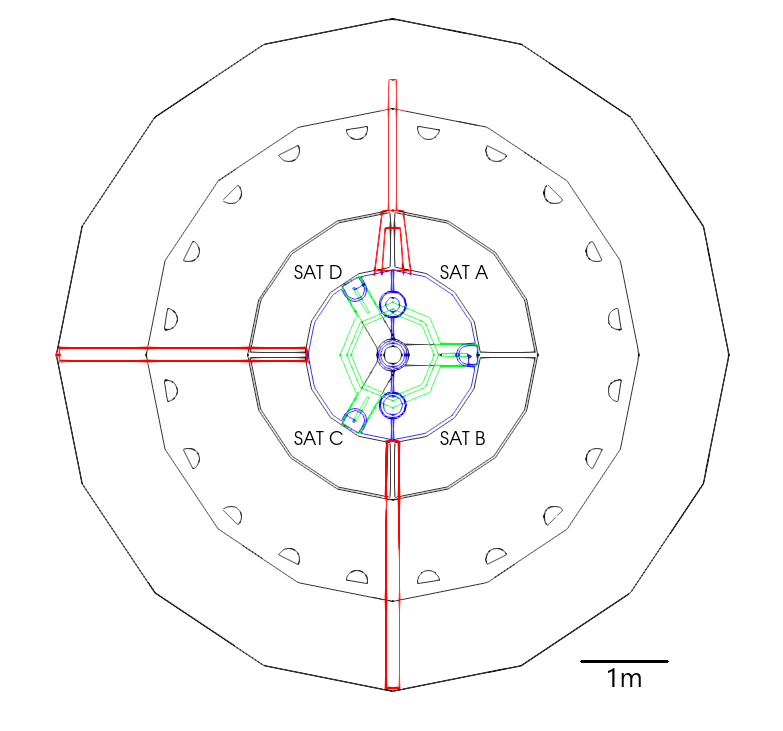
\includegraphics[width=\textwidth]{Figures/Geometry/geometry_with_conduits_with_scale.png}
\centering
\caption{LZ geometry schematic. The OD geometry, excluding the BATs and TATs is shown in black. The BATs and the bottom of the OCV are shown in green. The TATs, CSD ports and PMT conduits are shown in blue. The DD calibration conduits and the High-Voltage feed-through for the TPC are shown in red.}
\label{fig:OD_conduit_geometry}
\end{figure}


\begin{figure}[!htbp]
    \centering
    \begin{tikzpicture}
    
    \begin{axis}[
        xlabel=Pulse Area,
        ylabel=Rate (Hz/5phe),
        width=15cm, height=10cm,
        xmin=0, xmax=800,
        ymin=1e-4, ymode=log,
        legend pos=north east,
        grid=major]
            
        \addplot[only marks, mark size=0.5pt] 
            plot[error bars/.cd, x dir=both, x explicit]
            table[x=pulsearea,y=rate,x error=x_error, y error=y_error]
            {Data/OD_Backgrounds/background_constraints/od_data_pulsearea_middle_tank_binwidth_5.dat};
            
        \end{axis}
    \end{tikzpicture}
    \caption{OD pulse area spectrum from pulses reconstructed to the middle of the OD side tanks, suppressing the rate from Cavern-$\gamma$'s.}
    \label{fig:od_data_pulsearea_middle_tank}
\end{figure}


\subsection{$\gamma$ constraints}
\par
Another area to look at is high energy $\gamma$s from ($\alpha$,$\gamma$) reactions, which were discussed in \autoref{sec:cavern_gamma_generator}.
In \autoref{fig:od_high_energy} the expected and observed rate above 400 phd is shown.
The rate of events expected is significantly greater than that observed.
The findings here support the discussion in \autoref{sec:cavern_gamma_generator} that the statistical model used by GEANT4 does not extend well to ${}^{17}$O.
However, there are still events seen in data between 1000 and 1800~phd that are not accounted for in simulations.
These features have been attributed to neutron captures on the Fe of the water tank (which is made of steel), producing high energy $\gamma$s \cite{iron_neutrons_ref}.
These neutrons originate primarily from the ${}^{252}$Cf calibration source, which was stored in a movable safe underground during SR1.
The source was moved around within the cavern during SR1, which matches with a change in the reconstructed position of these events.
Backgrounds of this type were not previously considered within LZ, though are of great importance in fusion experiments \cite{iter_neutrons_ref}.
Due to the safe's placement during SR1, it was not possible to determine if there was any fluctuation in the high-energy $\gamma$ rate during SR1.

\begin{figure}[]
    \centering
    \begin{tikzpicture}
    
    \begin{axis}[
        xlabel=Pulse Area (phd),
        ylabel=Rate (Hz),
        width=15cm, height=10cm,
        xmin=400, xmax=3000,
        %ymax=1e-7, 
        ymode=log,
        legend pos=north east,
        grid=major]
            
        \addplot[only marks, mark size=0.5pt,
                 error bar legend,] 
            plot[error bars/.cd, x dir=both, x explicit]
            table[x=pulsearea,y=weight,x error=xerror, y error=yerror]
            {Data/OD_Backgrounds/background_constraints/od_data.dat};
            
        \addplot[red, const plot]
            table [x=pulsearea,y=weight]
            {Data/OD_Backgrounds/background_fit/starting_point/backgrounds_original_purification.dat};
            
        \legend{Data, Expectation};
        \end{axis}
    \end{tikzpicture}
    \caption{OD pulse area spectrum for high energy $\gamma$ events compared to the expected rate.
             The events observed in data between 1000 and 1800 phd are high energy $\gamma$-rays from neutron capture the iron.}
    \label{fig:od_high_energy}
\end{figure}

%%%%%%%%%%%%
\subsection{$\alpha$ constraints}
\par
As was discussed in \autoref{sec:simulated_od_backgrounds}, the exact rate of backgrounds from GdLS internals components is not known, as the improved purification cocktail was not assayed.
Fortunately, we are able to constrain some of the components. 
The decays within the U and Th decay chains all have an isotope in them with a half-life shorter than the LZ event window, of 4.5~ms.
It is, therefore, possible to observe two decays from the same decay chain, which will appear as two pulses (one from each decay) in an event.
There are three decay pairs for this, one from ${}^{238}$U, ${}^{235}$U, and ${}^{232}$Th.
These are summarised in \autoref{tab:od_constrainable_decays_in_data}.

\begin{table}[]
    \centering
    \begin{tabular}{c|c|c|c|c|c}
        \multirow{2}{*}{Decay Pair (chain)}                    & \multicolumn{2}{c|}{First Decay}   & \multicolumn{3}{c}{Second Decay}    \\ 
                                                               & Decay    & Energy (MeV) & Decay    & Energy (MeV) & half-life ($\mu$s) \\ \hline
        ${}^{214}$Bi${}^{214}$Po (${}^{238}$U$_{m}$)          & $\beta$  & 3.27         & $\alpha$ & 7.83         & 160   \\ 
        ${}^{219}$Rn${}^{215}$Po (${}^{235}$U$_{l}$)          & $\alpha$ & 6.95         & $\alpha$ & 7.53         & 1800  \\ 
        ${}^{212}$Bi${}^{212}$Po (${}^{232}$Th$_{l}$)         & $\beta$  & 2.25         & $\alpha$ & 8.95         & 0.3
    \end{tabular}
    \caption{Th and U decay chain pairs with half-lives within the LZ event window of 4.5 ms. 
             Decay information from \cite{radon_chains_ref}.
             See \autoref{fig:decay_chains} for the complete decay chains.}
    \label{tab:od_constrainable_decays_in_data}
\end{table}

\par
The decay pairs were searched for by looking for pulses which were reconstructed to be in close spatial proximity to each other.
As the GdLS is not circulated and the decay particles ($\beta$ and $\alpha$) do not have significant penetrating power, the site of the two interactions will be very close to each other.
Implementing a position requirement reduces the impact of accidental coincident signals in other areas of the OD being mistakenly identified as part of the pulse pair.
The data selection criteria used was simply requiring that the reconstructed $z$ and $\phi$ be within some range of each other: $z_{\text{diff}} < 25$ and $\phi_{\text{diff}} < 1.0$, where diff refers to the difference between the two pulses.
It was also limited to pulses passing the noise cut, ensuring that enough PMTs saw light to make the reconstruction meaningful.
This cut is fairly loose to account for potential inefficiencies in the position reconstruction.
The resultant pulse pairs are shown in \autoref{fig:od_all_pulse_pairs_2d}.
Only pulses above 200~keV in visible energy are included in the figure to make the features easier to see.

\begin{figure}[!htbp]%
\centering
\begin{tikzpicture}
\centering
  \begin{axis}[
    height=10cm, width=10cm,
    view={0}{90},
    ylabel={Second Pulse (phd)},
    xlabel={First Pulse (phd)},
    colorbar,
    colorbar style={ylabel={Rate (Hz)},ymode=log,},
    ]
    \addplot3[
      surf,
      shader=flat corner,
	  mesh/cols=40,
	  mesh/ordering=rowwise,
	  point meta = {z<0.0000001 ? nan : z}
    ] file {Data/OD_Backgrounds/background_constraints/rnpo_rate_2d.dat};

  \end{axis}
\end{tikzpicture}
\caption{Relationship of pulses reconstructed in close proximity to each other. Only pulses above 200 keV have been included.}
\label{fig:od_all_pulse_pairs_2d}
\end{figure}

\begin{figure}[!htbp]%
\centering
\begin{tikzpicture}
\centering
  \begin{groupplot}[%view={0}{90},
    group style = {group size = 1 by 2,vertical sep=1.5cm,
                   horizontal sep=1.5cm},
                   height=6cm, width=0.5\textwidth]

	\nextgroupplot[height=10cm, width=10cm,
    view={0}{90},
    ylabel={Second Pulse (phd)},
    xlabel={First Pulse (phd)},
    colorbar,
    colorbar style={ylabel={Rate (Hz)},ymode=log,},
    ]
    \addplot3[
      surf,
      shader=flat corner,
	  mesh/cols=40,
	  mesh/ordering=rowwise,
	  point meta = {z<0.0000001 ? nan : z}
    ] file {Data/OD_Backgrounds/background_constraints/rnpo_rate_2d.dat};
    
    
    \nextgroupplot[height=10cm, width=10cm,
    view={0}{90},
    ylabel={Second Pulse (phd)},
    xlabel={First Pulse (phd)},
    colorbar,
    colorbar style={ylabel={Rate (Hz)},ymode=log,},
    ]
    \addplot3[
      surf,
      shader=flat corner,
	  mesh/cols=40,
	  mesh/ordering=rowwise,
	  point meta = {z<0.0000001 ? nan : z}
    ] file {Data/OD_Backgrounds/background_constraints/bipo_rate_2d.dat};
   
  \end{groupplot}
\end{tikzpicture}
\caption{Relationship of pulses reconstructed in close proximity to each other. Only pulses above 200 keV have been included.
         \textbf{Top:} All pulses-pairs within 800 $\mu$s of each other. The distribution is from ${}^{214}$Bi $\to {}^{214}$Po.
         \textbf{Bottom:} All pulse-pairs with more than 800 $\mu$s time separation between them. The distribution left is from ${}^{219}$Rn $\to {}^{215}$Po.
         }
\label{fig:od_time_dependent_pulses_2d}
\end{figure}



\par
In \autoref{fig:od_all_pulse_pairs_2d}, there is a distribution where both the first and second pulse both have a signal size of around 170 phd.
This corresponds to the double $\alpha$-decay of ${}^{219}$Rn$\to{}^{215}$Po$\to{}^{211}$Pb.
The first pulse is slightly smaller than the second, which follows the pattern expected given the $\alpha$ energies shown in \autoref{tab:od_constrainable_decays_in_data}.
The other two pulse pairs will be spread out (in the $x$-axis) as the first pulses are from $\beta$-decays and so are not visible as features in \autoref{fig:od_all_pulse_pairs_2d}.
It is still possible to isolate these by taking advantage of the much shorter decay half-life of ${}^{212}$Po and ${}^{214}$Po compared to ${}^{215}$Po.
This was done by incorporating a time requirement, where the pulse pairs had to be within 320~$\mu$s of each other.
This time was chosen as it corresponds to 2 full half-lives of ${}^{214}$Po, in which 75\% of all ${}^{214}$Po will have decayed and is sufficiently lower than the half-life of ${}^{215}$Po so that its contribution will be minimal.
The result of this is shown in \autoref{fig:od_time_dependent_pulses_2d}.
The distribution centred at 240~phd (in the $y$-axis), corresponding to the $\alpha$-decay of ${}^{212}$Po.
The $\alpha$ from ${}^{214}$Po would be expected around 180~phd, but the rate is sufficiently low that it cannot be seen.

\par
Each sub-chain, ${}^{238}$U$_{m}$, ${}^{235}$U$_{l}$ and ${}^{232}$Th$_{l}$, is expected to contribute to the OD background rate via the two decays in the range [15, 192]~mHz, [20, 185]~mHz and [5, 50]~mHz respectively.
The lower bound on each expectation assumes that the GdLS underwent the improved purification (discussed in \autoref{sec:simulated_od_requirements}).
The upper bound assumes the rate is what was measured in the LS screener assay \cite{scotthaselschwardt_thesis_ref}.
The rates calculated here are 98$\pm$2.5~mHz for ${}^{219}$Rn$\to{}^{215}$Po$\to{}^{211}$Pb (${}^{235}$U$_{l}$) and 7.7$\pm$1.2~mHz for ${}^{212}$Bi$\to{}^{212}$Po$\to{}^{208}$Pb (${}^{232}$Th$_{l}$).
These were determined by isolating the feature in each distribution.
A second reverse search was also performed, where the $\alpha$ peak was found, and then the earlier first pulse was found, which provided an equivalent result.
As no feature was observed for ${}^{238}$U$_{m}$, it can be assumed that it does not contribute any significant rate.
The likely reason for this is that the improved purification worked especially well for removing that sub-chain.
Both the rates of ${}^{235}$U$_{l}$ and ${}^{232}$Th$_{l}$ are between the LS screener value and the improved purification estimate.
This indicates that the purification was performed but did not decrease all of the impurities as much as hoped for.
As the rates measured only included cases where both pulses were above 200~keV, the rate of ${}^{212}$Bi$\to{}^{212}$Po will be slightly higher given the $\beta$ spectrum of ${}^{212}$Bi. 
%There is efficiency of tagging ${}^{212}Bi \to {}^{212}Po$ is lower than that of ${}^{219}Rn \to {}^{215}Po$ as the half-life is only 300 ns.
%As can seen been in \autoref{fig:od_noise_cut_waveforms}, a pulse can last significantly longer than this.
%Therefore in order to be picked out, the pulses need to be far enough apart that the pulse finding algorithm can differentiate them.
%The signals are sampled at 10 ns so 

\par
The projections of the $\alpha$ pulses from \autoref{fig:od_all_pulse_pairs_2d} and \autoref{fig:od_time_dependent_pulses_2d} are shown in \autoref{fig:od_extracted_alphas}.
The signal size has been converted into visible energy according to the energy scale previously discussed.
The observed energy for each $\alpha$ was determined by a Gaussian fit to each peak.
The observed energy of each $\alpha$ versus the particle energy is shown in \autoref{fig:od_alpha_quenching}.
Included as well is the 2.2~MeV $\alpha$-decay from ${}^{152}$Gd that has been previously discussed.
The Birk's law expectation is also shown using the parameters in \autoref{tab:Birks_law_parameters}.
Each data point lines up in good agreement with the quenching parameters for pure LAB.
The parameters for quenching are used in the simulation chain, which further isolates the discrepancy in the OD response between simulations and observations to optical propagation in the simulation.
%The second point is the peak at 100 phd in \autoref{fig:od_random_trigger}, assuming that it's an $\alpha$-decay.
\par
In \autoref{fig:od_alpha_quenching}, an additional point is included from the peak at 100~phd in \autoref{fig:od_random_trigger}, assuming that it is an $\alpha$.
This indicates that it is likely from a $\backsim$5.4~MeV $\alpha$.
Turning back to \autoref{fig:decay_chains}, that is a fairly common $\alpha$ energy in all of the decay chains.
However, ${}^{238}$U$_{m}$, ${}^{235}$U$_{l}$ and ${}^{232}$Th$_{l}$ can all be ruled out as they do not have high enough rates.
The early chains of each decay chain can also be ruled out as the $\alpha$ decays are all below 5~MeV.
This opens up the possibility that it is a 5.3~MeV $\alpha$ from ${}^{210}$Po, which is in the late chain of ${}^{238}$U.
This suggestion appears at odds with the extremely low internal rate of ${}^{238}$U just measured.
However, it is known and measured that there is significant radon in the cavern air, and as previously discussed (\autoref{sec:od_construction_sec}), the acrylic tanks were open to the cavern air for long periods prior to filling.
There was an opportunity for decay daughters to plate-out on the inside of the acrylic tanks, a feature that is of great concern within the TPC \cite{radon_plateout_ref} (which was discussed in \autoref{sec:lz_detector}).
${}^{210}$Pb is the only long-lived particle in any of the decay chains after radon, with a half-life in excess of 22 years. 
The remainder of the isotopes would drastically reduce in abundance after a few weeks, leaving only ${}^{210}$Pb daughters visible at a sustained rate.
This allows the acrylic holding the scintillator to act as a reservoir, providing a constant supply of $\alpha$ decays from ${}^{210}$Po.
LZ is not alone in having experienced this, with KamLAND measuring a higher than expected rate of ${}^{238}$U$_l$ decays as well \cite{KamLAND_LS_contaminants_ref}.

\begin{figure}[!htbp]%
\centering
\begin{tikzpicture}
\centering
    \begin{axis}[
            ylabel=Rate (Hz/2keV),
            xlabel=Energy (MeV),
            width=15cm,
            height=8cm,
            grid=major,
            xmin=0, xmax=3,
            ymin=1e-4, ymode=log,]
            
        \addplot[red, only marks, mark size=1, 
                 error bars/.cd,
                 y dir=both, y explicit, error bar style={color=black}]
            table [x=energy,y=rate,y error plus index=2, y error minus index=3]
            {Data/OD_Backgrounds/background_constraints/od_bipo_first_alpha.dat};
            
        \addplot[blue, only marks, mark size=1, 
                 error bars/.cd,
                 y dir=both, y explicit, error bar style={color=black}]
            table [x=energy,y=rate,y error plus index=2, y error minus index=3]
            {Data/OD_Backgrounds/background_constraints/od_bipo_second_alpha.dat};
                
    \end{axis}
            
\end{tikzpicture}
    \caption{$\alpha$ energies in from BiPo and RnPo.}
    \label{fig:od_bipo_alphas}
\end{figure}

\begin{figure}[!htbp]%
\centering
\begin{tikzpicture}
\centering
    \begin{axis}[
            ylabel=Visible Energy (MeV),
            xlabel=Particle Energy (MeV),
            width=15cm,
            height=8cm,
            grid=major,
            xmin=0, xmax=10,
            ymin=0,
            legend pos=north west,
            ]
            
        % Birks Fit
        \addplot[red]
            table [x=Energy,y=Quenched]
            {Data/GdLS_Physics/Quenching/alpha.dat};
        \addplot[black, only marks, mark size=1, 
                 error bars/.cd, error bar style={color=black},
                 y dir=both, y explicit,]
            table [x=energy,y=observed,y error plus index=2, y error minus index=3]
            {Data/OD_Backgrounds/background_constraints/od_alpha_energies.dat};
        \legend{Birk's, Measured};
    \end{axis}
            
\end{tikzpicture}
    \caption{Observed energy vs particle energy from $\alpha$ particles.
             The expected quenching from Birk's Law using the parameters in \autoref{tab:Birks_law_parameters} is shown to be in good agreement with what is observed.}
    \label{fig:od_alpha_quenching}
\end{figure}




\subsection{${}^{152}$Gd}
\par
The final background that can be constrained is ${}^{152}$Gd.
The GdLS is loaded with 0.1\% (by mass) of natural gadolinium.
The total mass of GdLS used in the detector is 16638~kg.
With a natural abundance of 0.2\% of ${}^{152}$Gd, this gives a maximum possible rate of 27Hz, with a 5\% uncertainty from the doping by mass.
Unfortunately, this does not constrain the contributions to the shoulder in \autoref{fig:od_random_trigger}.
As previously discussed, there are two other decays of note, ${}^{14}$C, a $\beta$ decay with an end-point of 156~keV, and ${}^{147}$Sm which decays via the emission of a 2.3~MeV $\alpha$.
All three were measured in the LS Screener assay and would not have changed with an improved purification \cite{scotthaselschwardt_thesis_ref}.
This means that the rate of these components scales only by the mass of GdLS.

%All three were previously measured in the LS screener campaign, with ${}^{14}$C being the dominant contributor \cite{scotthaselschwardt_thesis_ref}.
%This does not mean that ${}^{152}$Gd and ${}^{147}$Sm can be ignored, as

\subsection{Background Fitting}
\par
Using all of the information on the OD backgrounds discussed so far in this section, we finish with a fit of the expected backgrounds to what is observed.
Full chain simulations of all of the backgrounds identified in \autoref{sec:simulated_od_backgrounds} were performed with every signal scaled by 4.54.
Rather than fitting to the full observable space, a sub-range was defined between 20~phd and 600~phd.
The lower limit was set to be far enough away from the noise cut that any uncertainty in the scaling factor would not remove these events.
The upper limit was set by the point where the predicted rate of cavern-$\gamma$s diverged from the observation.
In this region, the expected background rate is 78.43$\pm$2.51~Hz.
This is slightly below the observed rate of 85.26$\pm$0.22~Hz.
\par
A fit was performed using RooFit \cite{roostats_ref}, where the contribution of each background component was allowed to float within a defined range.
In order to keep the number of fit parameters small a number of steps were taken.
Firstly, contributions from all detector components were combined.
This means that the spectra of each sub-component were summed, with the shape fixed but the magnitude variable.
${}^{60}$Co decay from the OCV is the most significant contributor here.
Secondly, contributions from ${}^{152}$Gd and ${}^{147}$Sm were combined as the energy resolution is not sufficient to separate them.
Cavern-$\gamma$s were allowed to float within the uncertainties measured in \cite{LZ_Gamma_Ray_Background_ref}.
${}^{238}$U$_l$ was allowed to float in the range of [0, 15]~Hz, where 15 is roughly double the size of the integrated rate of the peak at 100~phd above the rest of the spectra.
${}^{238}$U$_{m}$ and ${}^{235}$U$_{l}$ were constrained by the rates measured earlier.
All other backgrounds were allowed to float up to the maximum value measured in the LS screener campaign \cite{scotthaselschwardt_thesis_ref}.
The shape of each spectrum was fixed with only the integrated rate variable.
\par
The result of the fit is shown in \autoref{fig:od_background_fit_to_data}.
Only components that contributed more than 0.5~Hz to the OD rate are included in \autoref{fig:od_background_fit_to_data}, but the fitted line shows the contributions from all components.
The individual fitted rates for each component are shown in \autoref{tab:od_constrainable_decays_in_data}.
Included as well in \autoref{tab:od_constrainable_decays_in_data} is the rate of each component from the initial assumption from an improved purification case.
\par
Generally, there is good agreement between the fit and what was observed with a $\chi^2$/ndf = 212.6/135.
There is a difference of less than 10\% over most of the range with the main features of the distribution captured.
The most significant difference is at 50~phd where no background appears to be able to fill in this region.
This is likely an uncertainty from the scaling factor.
The flat scaling of 4.54 did not take into account any position variation.
Given that the light collection efficiency observed is significantly greater than simulated, it is logical to suggest that the variation in the light collection efficiency (shown in \autoref{fig:od_lce}) is also different.
This would effectively make contributions in lower light collection regions appear smaller than they are observed to be, which may go some way to explain the difference.
Without further calibrations, incorporating a variation in spectral shape is exceptionally complicated.
\par
The cavern-$\gamma$s remain the highest contributor to the OD background rate, contributing to the rate across the entire phd range.
The rate from cavern-${}^{238}$U has increased to fill the background shape at 300~phd.
At low phd values, the dominating contribution is from ${}^{14}$C, with the rate being very close to what was expected.
The rate of ${}^{152}$Gd and ${}^{147}$Sm has decreased, but this could equally have been done to ${}^{14}$C.
There is little to differentiate between these sources in the fit region.
${}^{238}$U$_l$ can successfully account for the peak observed at 100~phd, contributing over 8~Hz to the OD rate.
\par
Many low-rate decays have not changed between the expected rate and the fit.
This is due to the domination of a few background components.
After future calibrations, it will be possible to include these more meaningfully by suppressing the cavern-$\gamma$s as previously discussed.
Regardless, this first attempt at measuring the background rates in the OD demonstrates that the components are well understood with the key features identified.

\begin{figure}[!htbp]%
\centering
\begin{tikzpicture}
\centering
    \begin{groupplot}[
    group style = {group size = 1 by 2,vertical sep=1.0cm}
    ]
    \nextgroupplot[
            ylabel=Rate (Hz/5phd),
            xlabel=,
            xmajorticks=false,
            width=15cm,
            height=10cm,
            grid=major,
            xmin=0, xmax=700,
            ymin=1e-2, ymax=100,
            ymode=log,
            legend style = { column sep = 10pt, legend columns = 3, cells={line width=1.5pt}}
            ]
        \addplot[only marks, mark size=1.0pt, black, error bar legend] 
            plot[error bars/.cd, x dir=both, x explicit, ]%y dir=both, y explicit, ]
            table[x=pulsearea,y=weight,x error=xerror, y error=yerror]
            {Data/OD_Backgrounds/background_constraints/od_data.dat};
        \addlegendentry{data};
            
        \addplot[const plot, teal]
            table [x=bin_low, y=weight]
            {Data/OD_Backgrounds/background_fit/fit_components/rg_k40.dat};
        \addlegendentry{Cavern ${}^{40}$K};
        \addplot[const plot, cyan]
            table [x=bin_low, y=weight]
            {Data/OD_Backgrounds/background_fit/fit_components/rg_u238.dat};
        \addlegendentry{Cavern ${}^{238}$U};
        \addplot[const plot, green]
            table [x=bin_low, y=weight]
            {Data/OD_Backgrounds/background_fit/fit_components/rg_th232.dat};
        \addlegendentry{Cavern ${}^{232}$Th};
        \addplot[const plot, lime]
            table [x=bin_low, y=weight]
            {Data/OD_Backgrounds/background_fit/fit_components/ocv.dat};
        \addlegendentry{Detector};
        \addplot[const plot, yellow]
            table [x=bin_low, y=weight]
            {Data/OD_Backgrounds/background_fit/fit_components/Internal_improved_u238_early.dat};
        \addlegendentry{${}^{238}$U early};
        \addplot[const plot, pink]
            table [x=bin_low, y=weight]
            {Data/OD_Backgrounds/background_fit/fit_components/Internal_improved_u238_late.dat};
        \addlegendentry{${}^{238}$U late};    
        \addplot[const plot, olive]
            table [x=bin_low, y=weight]
            {Data/OD_Backgrounds/background_fit/fit_components/Internal_improved_th232_early.dat};
        \addlegendentry{${}^{232}$Th early};
        \addplot[const plot, brown]
            table [x=bin_low, y=weight]
            {Data/OD_Backgrounds/background_fit/fit_components/Internal_improved_C14.dat};
        \addlegendentry{${}^{14}$C};
        \addplot[const plot, orange]
            table [x=bin_low, y=weight]
            {Data/OD_Backgrounds/background_fit/fit_components/Internal_improved_Gd152.dat};
        \addlegendentry{${}^{152}$Gd + ${}^{147}$Sm};
        \addplot[const plot, violet]
            table [x=bin_low, y=weight]
            {Data/OD_Backgrounds/background_fit/fit_components/total_fit.dat};
        \addlegendentry{fit};
            
            
    \nextgroupplot[
            ylabel=Ratio (data/fit),
            xlabel=Pulse Area (phd),
            width=15cm,
            height=5cm,
            grid=major,
            xmin=0, xmax=700,
            ymin=0, ymax=2,
            ]
        \addplot[only marks, mark size=1.0pt, black, error bar legend] 
            plot[error bars/.cd, y dir=both, y explicit]
            table[x=bin,y=value, y error=error]
            {Data/OD_Backgrounds/background_fit/fit_components/ratio.dat};
        
        \addplot[black, mark=none, dashed] coordinates {(20,-1) (20,3)};
        \addplot[black, mark=none, dashed] coordinates {(600,-1) (600,3)};
        
    \end{groupplot}
\end{tikzpicture}
    \caption{Result of fit to data.
             \textbf{Top:} Contribution from each source. Only components with a contribution greater than 1 Hz have been included.
             \textbf{Bottom:} Ratio of fit to data. The dashed lines indicate the fit region.
             In generally there is good agreement.}
    \label{fig:od_background_fit_to_data}
\end{figure}


\begin{table}[]
    \centering
    \begin{tabular}{c|c|c|c}
        Source               &  Decay Type(s)               & Estimated Rate (Hz) & Fitted Rate (Hz) \\ \hline
        \multicolumn{4}{l}{\textbf{Externals}} \\
        Cavern ${}^{40}$K    & $\gamma$                     & 6.61$\pm$1.98       & 7.65$\pm$0.55                    \\ 
        Cavern ${}^{232}$Th  & $\gamma$                     & 13.79$\pm$3.17      & 12.94$\pm$2.04                    \\ 
        Cavern ${}^{238}$U   & $\gamma$                     & 10.63$\pm$5.53      & 12.50$\pm$1.77                    \\ 
        Detector             & $\gamma$,$\beta$             & 2.16$\pm$2.67       & 3.63$\pm$0.67              \\ \hline
        \multicolumn{4}{l}{\textbf{Internals}} \\
        ${}^{238}$U$_{e}$     & $\gamma$,$\alpha$,$\beta$   & 0.68$\pm$0.31       & 0.98$\pm$0.21                    \\ 
        ${}^{238}$U$_{m}$     & $\gamma$,$\alpha$,$\beta$   & 0.30$\pm$0.10       & 0.03$\pm$0.10                   \\
        ${}^{238}$U$_{l}$     & $\gamma$,$\alpha$,$\beta$   & 0.11$\pm$0.11       & 8.74$\pm$2.34                \\
        ${}^{235}$U$_{e}$     & $\gamma$,$\alpha$,$\beta$   & 0.71$\pm$0.33       & 0.39$\pm$0.23                    \\
        ${}^{235}$U$_{l}$     & $\gamma$,$\alpha$,$\beta$   & 0.32$\pm$0.15       & 0.44$\pm$0.12                    \\
        ${}^{232}$Th$_{e}$    & $\gamma$,$\alpha$,$\beta$   & 0.12$\pm$0.07       & 0.18$\pm$0.04                    \\
        ${}^{232}$Th$_{l}$    & $\gamma$,$\alpha$,$\beta$   & 0.24$\pm$0.09       & 0.51$\pm$0.08                  \\
        ${}^{40}$K          & $\gamma$,$\beta$              & 0.05$\pm$0.01       & 0.05$\pm$0.01                 \\
        ${}^{14}$C          & $\beta$                       & 27.22$\pm$12.24     & 26.97$\pm$7.70           \\
        ${}^{176}$Lu        & $\gamma$,$\beta$              & 0.16$\pm$0.08       & 0.14$\pm$0.05               \\
        ${}^{147}$Sm and ${}^{152}$Gd    & $\alpha$         & 16.22$\pm$7.24      & 10.32$\pm$5.24                     
        
    \end{tabular}
    \caption{Fitting contributions of OD backgrounds to the observed data. 
             The estimated rates are from the improved purification assumption.
             The reported errors in the fit are statistical only.}
    \label{tab:od_fitted_background_rates}
\end{table}
